\documentclass{article}

\usepackage{fancyhdr}
\usepackage{extramarks}
\usepackage{amsmath}
\usepackage{amsthm}
\usepackage{amsfonts}
\usepackage{tikz}
\usepackage[plain]{algorithm}
\usepackage{algpseudocode}
\usepackage{graphicx}
\usepackage{epstopdf}
\usepackage{xfrac}
\usepackage{siunitx}
\usepackage[americanvoltages]{circuitikz}


\usetikzlibrary{automata,positioning}

%
% Basic Document Settings
%

\topmargin=-0.45in
\evensidemargin=0in
\oddsidemargin=0in
\textwidth=6.5in
\textheight=9.0in
\headsep=0.25in

\linespread{1.1}

\pagestyle{fancy}
\lhead{\hmwkAuthorName}
\chead{\hmwkClass\ (\hmwkClassInstructor\ \hmwkClassTime): \hmwkTitle}
\rhead{\firstxmark}
\lfoot{\lastxmark}
\cfoot{\thepage}

\renewcommand\headrulewidth{0.4pt}
\renewcommand\footrulewidth{0.4pt}

\setlength\parindent{0pt}

%
% Create Problem Sections
%

\newcommand{\enterProblemHeader}[1]{
    \nobreak\extramarks{}{Problem \arabic{#1} continued on next page\ldots}\nobreak{}
    \nobreak\extramarks{Problem \arabic{#1} (continued)}{Problem \arabic{#1} continued on next page\ldots}\nobreak{}
}

\newcommand{\exitProblemHeader}[1]{
    \nobreak\extramarks{Problem \arabic{#1} (continued)}{Problem \arabic{#1} continued on next page\ldots}\nobreak{}
    \stepcounter{#1}
    \nobreak\extramarks{Problem \arabic{#1}}{}\nobreak{}
}

\setcounter{secnumdepth}{0}
\newcounter{partCounter}
\newcounter{homeworkProblemCounter}
\setcounter{homeworkProblemCounter}{1}
\nobreak\extramarks{Problem \arabic{homeworkProblemCounter}}{}\nobreak{}

%
% Homework Problem Environment
%
% This environment takes an optional argument. When given, it will adjust the
% problem counter. This is useful for when the problems given for your
% assignment aren't sequential. See the last 3 problems of this template for an
% example.
%
\newenvironment{homeworkProblem}[1][-1]{
    \ifnum#1>0
        \setcounter{homeworkProblemCounter}{#1}
    \fi
    \section{Problem \arabic{homeworkProblemCounter}}
    \setcounter{partCounter}{1}
    \enterProblemHeader{homeworkProblemCounter}
}{
    \exitProblemHeader{homeworkProblemCounter}
}

%
% Homework Details
%   - Title
%   - Due date
%   - Class
%   - Section/Time
%   - Instructor
%   - Author
%

\newcommand{\hmwkTitle}{Assignment\ 2}
\newcommand{\hmwkDueDate}{May 5, 2017}
\newcommand{\hmwkClass}{Power Systems Analysis}
\newcommand{\hmwkClassTime}{}
\newcommand{\hmwkClassInstructor}{Kamal Debnath}
\newcommand{\hmwkAuthorName}{S.Reynolds (262538)}

%
% Title Page
%

\title{
    \vspace{2in}
    \textmd{\textbf{\hmwkClass:\ \hmwkTitle}}\\
    \normalsize\vspace{0.1in}\small{Due\ on\ \hmwkDueDate\ at 3:00pm}\\
    \vspace{0.1in}\large{\textit{\hmwkClassInstructor\ \hmwkClassTime}}
    \vspace{3in}
}

\author{\textbf{\hmwkAuthorName}}
\date{}

\renewcommand{\part}[1]{\textbf{\large Part \Alph{partCounter}}\stepcounter{partCounter}\\}

%
% Various Helper Commands
%

% Useful for algorithms
\newcommand{\alg}[1]{\textsc{\bfseries \footnotesize #1}}

% For derivatives
\newcommand{\deriv}[1]{\frac{\mathrm{d}}{\mathrm{d}x} (#1)}

% For partial derivatives
\newcommand{\pderiv}[2]{\frac{\partial}{\partial #1} (#2)}

% Integral dx
\newcommand{\dx}{\mathrm{d}x}

% Alias for the Solution section header
\newcommand{\solution}{\textbf{\large Solution}}

% Probability commands: Expectation, Variance, Covariance, Bias
\newcommand{\E}{\mathrm{E}}
\newcommand{\Var}{\mathrm{Var}}
\newcommand{\Cov}{\mathrm{Cov}}
\newcommand{\Bias}{\mathrm{Bias}}

\begin{document}

\maketitle

\pagebreak

\begin{homeworkProblem}

Consider the single-phase two-wire solid conductor in Figure 1. The distance between the centres of the wires is $d$, and each wire has a radius of $r$. Now, if the two wires form a single rectangular loop, then at any instance we know that the currents in the wire 1, $I_1$, flows in the opposite direction to the current in wire 2, $I_2$. That is to say that $I_1 = -I_2$. We note that the magnitude of the currents are equal, say $I$. Considering wire 1, we note that there are two flux linkages that are established. The first is the flux linkage that the wire has with itself, $\lambda_{11}$, which is found by considering a point that falls a distance of less than $r$ away from the wire. The second flux linkage on wire 1 is established due to the second wire. We call this $\lambda_{12}$, and is found by considering a distance of some point from the wire which is greater than $r$, but less than $d + r$. There is a third case to consider, where the distance is greater than $d + r$, however, we note that in this instance there is no flux linkage established because the current is flowing in opposite directions and of equal magnitude.\\

\begin{figure}[H]
\centering
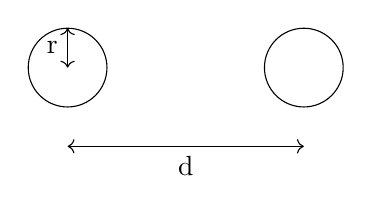
\begin{tikzpicture}
	\draw (0,0) circle (0.5cm);
	\draw (3,0) circle (0.5cm);
	\draw [<->] (0,0)--(0,0.5) node[midway,left]{r};
	\draw [<->] (0,-1)--(3,-1) node[midway,below]{d};
\end{tikzpicture}
\caption{Two solid conductors forming a loop}
\end{figure}

Now the internal flux linkage is given by:
\begin{align*}
	\lambda_{11} = \frac{1}{2} \times I \times 10^{-7}
\end{align*}

The external flux linkage is given by:
\begin{align*}
	\lambda_{12} = 2 \times 10^{-7} \times I \ln (\frac{d-r}{r})
\end{align*}

The total flux linkage on wire 1 is found simply by adding the internal and external flux linkages:
\begin{align*}
	\lambda_1   &= \lambda_{11} + \lambda_{12}\\
				&= \frac{1}{2} \times I_1 \times 10^{-7} + 2 \times 10^{-7} \ln \big(\frac{d-r}{r} \big)\\
				&= 10^{-7} \cdot \big[\frac{1}{2} + 2 \times I \times \ln \big(\frac{d-r}{r} \big)\big]\\
				&= I \cdot \bigg(\frac{1}{2} \times 10^{-7} \cdot \big[ 1 + 4 \ln \big(\frac{d-r}{r} \big) \big] \bigg)
\end{align*}

Now, the inductance on wire one is given by:
\begin{align*}
	L_1 = \frac{\lambda_1}{I} = \frac{1}{2} \times 10^{-7} \cdot \big[ 1 + 4 \ln \big(\frac{d-r}{r} \big) \big]
\end{align*}
\end{homeworkProblem}

Given that the problem is symmetrical we reason that $L_1 = L_2$. Further, the total inductance is given by adding the inductance from wire 1 to the inductance form wire 2, that is:
\begin{align*}
	L_{total} 	&= L_1 + L_2\\
				&= \frac{1}{2} \times 10^{-7} \cdot \big[ 1 + 4 \ln \big(\frac{d-r}{r} \big) \big] + \frac{1}{2} \times 10^{-7} \cdot \big[ 1 + 4 \ln \big(\frac{d-r}{r} \big) \big]\\
				&= 10^{-7} \cdot \big[ 1 + 4 \ln \big(\frac{d-r}{r} \big) \big]\\
				&= \frac{4 \pi}{4 \pi} \times 10^{-7} \cdot \big[ 1 + 4 \ln \big(\frac{d-r}{r} \big) \big]\\
				&= \frac{\mu_0}{4 \pi} \cdot \big[ 1 + 4 \ln \big(\frac{d-r}{r} \big) \big]
\end{align*}

\begin{homeworkProblem}

Calculation of transmission line parameters for stranded cables requires that we make approximations of the average distances between strands both within the transmission line itself, and between strands of two, individual stranded conductors.

\begin{figure}[H]
\centering
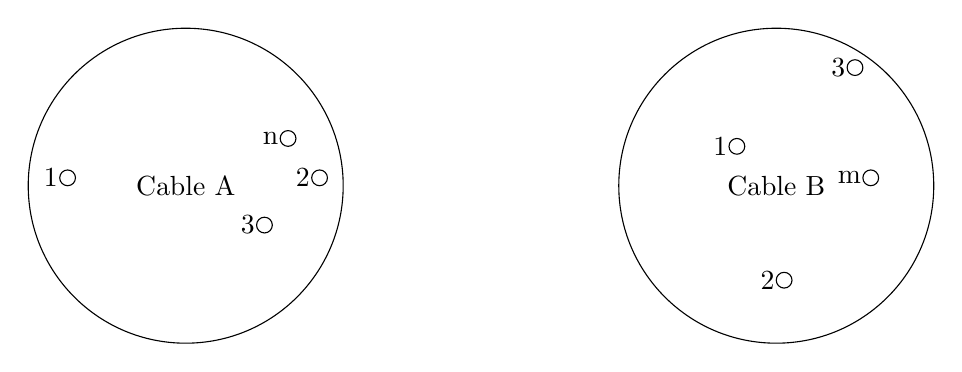
\begin{tikzpicture}
	\draw (0,0) circle (2cm) node[]{Cable A};
	\draw (7.5,0) circle (2cm) node[]{Cable B};
	
	\draw (-1.5,0.1) circle (0.1cm) node[left]{1};
	\draw (1.7,0.1) circle (0.1cm) node[left]{2};
	\draw (1,-0.5) circle (0.1cm) node[left]{3};
	\draw (1.3,0.6) circle (0.1cm) node[left]{n};
	
	\draw (7.5+-0.5,0.5) circle (0.1cm) node[left]{1};
	\draw (7.5+0.1,-1.2) circle (0.1cm) node[left]{2};
	\draw (7.5+1,1.5) circle (0.1cm) node[left]{3};
	\draw (7.5+1.2,0.1) circle (0.1cm) node[left]{m};
	
\end{tikzpicture}
\caption{Two stranded cables - cable A has $n$ strands and cable B has $m$ strands}
\end{figure}

To find the distances between strands in a single conductor (that is a single transmission line) we use the GMR which is also known as $D_s$ in some texts. Consider cable A shown in Figure 2. We see that there are $n$ strands and therefore $n^2$ distances to consider. To find $D_s$ we use the following formula:
\begin{align*}
	GMR = D_s = \sqrt[n^2]{(r' d_{12} d_{13} ... d_{1n}) ... (r' d_{n1} d_{n2} ... d_{(n-1)n})}
\end{align*}

To find the distances between two conductors which consist of multiple strands, we use GMD which is also known as $D_m$ in some texts. Consider both cable A and B shown in Figure 2. We see that there are $n$ strands in cable A and m strands in cable B. Now, for GMD we define $d_{11}$ as the distance between strand 1 in cable A and strand 1 in cable B; $d_{12}$ as the distance between strand 1 in cable A and strand 2 in cable B; $d_{21}$ as the distance between strand 2 in cable A and strand 1 in cable B, and so on. Hence, we get the following formula:
\begin{align*}
	GMD = D_m = \sqrt[mn]{(d_{11} d_{12} ... d_{1m})(d_{21} d_{22} ... d_{2m})...(d_{n1} d_{n2}...d_{nm})}
\end{align*}  
 
 \newpage
 
\textbf{Part A}\\
Consider a single conductor which consists of 2 strands as shown in Figure 3.

\begin{figure}[H]
\centering
	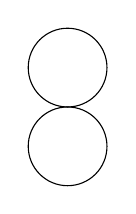
\begin{tikzpicture}
		\draw (0,0) circle (0.5cm);
		\draw (0,1) circle (0.5cm);
	\end{tikzpicture}
	\caption{A single conductor with 2 strands.}
\end{figure}

We note that $n = 2$, and that:
\begin{align*}
	GMR &= \sqrt[2^2]{(r' \cdot d_{12})(r' \cdot d_{21})}
\end{align*}
 
We note that $r' = 0.7788r$ and that $d_{12} = d_{21} = 2r$, and hence:
\begin{align*}
 	GMR &= \sqrt{0.7788r \cdot 2r}\\
 		&= 1.248r
\end{align*}

\textbf{Part B}\\
Consider the single conductor which consists of 3 strands as shown in Figure 4.

\begin{figure}[H]
\centering
	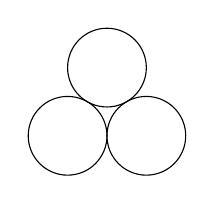
\begin{tikzpicture}
		\draw (0,0) circle (0.5cm);
		\draw (1,0) circle (0.5cm);
		\draw (0.5,0.86602) circle (0.5cm);
	\end{tikzpicture}
	\caption{A single conductor with 3 strands.}
\end{figure}

We note that $n = 3$, and that:
\begin{align*}
	GMR = \sqrt[3^2]{(r'd_{12}d_{13})(r'd_{21}d_{23})(r'd_{31}d_{32})}
\end{align*}

We note that $r' = 0.7788r$ and that all of the distances are the same and are $2r$ in length. Then we get:
\begin{align*}
	GMR &= \sqrt[9]{(r')^3 \cdot (2r)^6}\\
		&= \sqrt[9]{(0.7788)^3 \cdot 2^6} \cdot r\\
		&= 1.46 r
\end{align*}

\textbf{Part C}\\
Consider the single conductor which consists of 3 strands as shown in Figure 5.

\begin{figure}[H]
\centering
	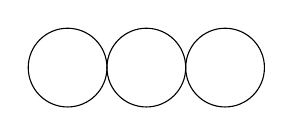
\begin{tikzpicture}
		\draw (0,0) circle (0.5cm);
		\draw (1,0) circle (0.5cm);
		\draw (2,0) circle (0.5cm);
	\end{tikzpicture}
	\caption{A single conductor with 3 strands.}
\end{figure}

We note that $n = 3$, and that:
\begin{align*}
	GMR = \sqrt[3^2]{(r'd_{12}d_{13})(r'd_{21}d_{23})(r'd_{31}d_{32})}
\end{align*}

We note that $r' = 0.7788r$, and that $d_{12} = d_{21} = d_{32} = d_{23} = 2r$, and that $d_{13} = d_{31} = 4r$. Hence, we see that:
\begin{align*}
	GMR &= \sqrt[9]{(r')^3\cdot (2r)^4 \cdot (4r)^2}\\
		&= \sqrt[9]{(0.7788)^3 \cdot 2^4 \cdot 4^2} \cdot r\\
		&= 1.703r
\end{align*}

\textbf{Part D}\\
Consider the single conductor which consists of 3 strands as shown in Figure 6.

\begin{figure}[H]
\centering
	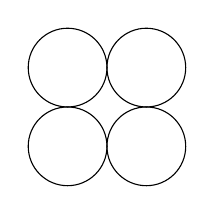
\begin{tikzpicture}
		\draw (0,0) circle (0.5cm);
		\draw (1,0) circle (0.5cm);
		\draw (0,1) circle (0.5cm);
		\draw (1,1) circle (0.5cm);
	\end{tikzpicture}
	\caption{A single conductor with 4 strands.}
\end{figure}

We note that $n = 4$, and that:
\begin{align*}
	GMR = \sqrt[4^2]{(r'd_{12}d_{13}d_{14})(r'd_{21}d_{23}d_{24})(r'd_{31}d_{32}d_{34})(r'd_{41}d_{42}d_{43})}
\end{align*}

We note that $r' = 0.7788r$, and that given the geometric symmetry in the problem there are 2 distances that are $2r$, and a single distance of $2\sqrt{2}r$. Hence, we get that:
\begin{align*}
	GMR &= \sqrt[16]{(r')^4 \cdot (2r)^4 \cdot (2r)^4 \cdot (2\sqrt{2}r)^4}\\
		&= \sqrt[16]{(0.7788)^4 \cdot 2^4 \cdot 2^4 \cdot 2^4 \cdot (\sqrt{2})^4} \cdot r\\
		&= 1.72r
\end{align*}

\textbf{Part E}\\
Consider the single conductor which consists of 3 strands as shown in Figure 7.

\begin{figure}[H]
\centering
	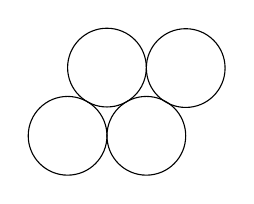
\begin{tikzpicture}
			\draw (0,0) circle (0.5cm);
			\draw (1,0) circle (0.5cm);
			\draw (0.5,0.86602) circle (0.5cm);
			\draw (1.5,0.86) circle (0.5cm);
		\end{tikzpicture}
		\caption{A single conductor with 4 strands.}
\end{figure}

We note that $r' = 0.7788r$, and that given the geometric symmetry in the problem there are 2 strands which have distances that are all $2r$, and 2 strands which have 2 distances of $2r$ and a single distance of $2\sqrt{3}r$. Hence, we get that:
\begin{align*}
	GMR &= \sqrt[4^2]{(r')^4 \cdot (2r \cdot 2r \cdot 2r )^2 \cdot (2r \cdot 2r \cdot 2 \sqrt{3})^2}\\
		&= \sqrt[16]{0.7788^4 \cdot (2)^6 \cdot (2)^4 \cdot (2 \sqrt{3})^2} \cdot r\\
		&= 1.692r
\end{align*}

\newpage

\textbf{Part F}\\
Consider the single conductor which consists of 7 strands in a circular pattern with one strand at the centre. In this instance, we have the following:
\begin{align*}
	GMR &= \sqrt[49]{0.7788^4 \cdot 2^18 \cdot (\sqrt{3})6{12} \cdot 4^6 \cdot 2^6} \cdot r\\
		&= 1.83r
\end{align*}


\end{homeworkProblem}

\begin{homeworkProblem}

Consider the three phase line shown in Figure 8. The solid lines are arranged in an equilateral triangle. Assuming that the three phase lines are balanced, it must be that $I_a + I_b + I_c = 0$. A point $M$ external to the conductors is also shown in Figure 3. The distances of the point from the phases a, b, and c are denoted by $D_{ma}$, $D_{mb}$, and $D_{mc}$. We note that the flux linked by the conductor a due to current $I_a$ includes the internal flux linkages but excludes the flux linkages beyond the point $m$. From the result we found in question 1 of this assignment, we note that:

\begin{figure}[H]
\centering
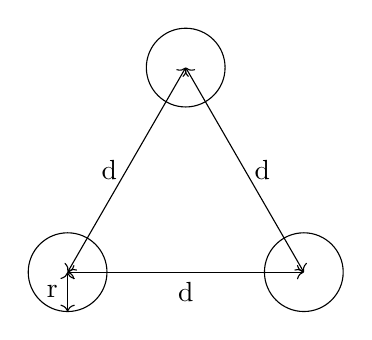
\begin{tikzpicture}
	\draw (0,0) circle (0.5cm);
	\draw (3,0) circle (0.5cm);
	\draw (1.5,2.598) circle (0.5cm);
	\draw [<->] (0,0) -- (0,-0.5) node[midway,left]{r};
	\draw [<->] (0,0) -- (1.5,2.598) node[midway,left]{d};
	\draw [<->] (0,0) -- (3,0) node[midway,below]{d};
	\draw [<->] (1.5,2.598) -- (3,0) node[midway,right]{d};
\end{tikzpicture}
\caption{Three solid conductors for a single phase, positioned with equal spacing between them.}
\end{figure}

\begin{align*}
	\lambda_{ma,a} = \frac{1}{2} \cdot I_a \cdot 2 \times 10^{-7} + 2 \times 10^{-7} \cdot I_a \cdot \ln(\frac{d_{pa} - r}{r})
\end{align*}

We note that $d \gg r$ and we instead write:
\begin{align*}
	\lambda_{ma,a} &= (\frac{1}{2} \times 10^{-7}) \cdot I_a \cdot \big(1 + 4 \ln \bigg(\frac{d_{pa}}{r}\bigg)\big)\\
				 &= (4 \cdot \frac{1}{2} \times 10^{-7}) \cdot I_a \cdot \big(\frac{1}{4} + \ln \bigg(\frac{d_{pa}}{r}\bigg)\big)\\
				 &= (2 \times 10^{-7}) \cdot I_a \cdot \big(\frac{1}{4} \cdot \ln (e) + \ln \bigg(\frac{d_{pa}}{r}\bigg)\big)\\
				 &= (2 \times 10^{-7}) \cdot I_a \cdot \big(\ln \bigg(\frac{d_{pa}}{r \cdot e^{-\frac{1}{4}}}\bigg)\big)\\
				 &= (2 \times 10^{-7}) \cdot I_a \cdot \ln \bigg(\frac{d_{pa}}{r'}\bigg)\\
\end{align*}

Hence, we see that:
\begin{align*}
	\lambda_{ap,a} = (2 \times 10^{-7}) \cdot I_a \cdot \ln \bigg(\frac{d_{pa}}{r'}\bigg)
\end{align*}

This is the flux of conductor a due to the conductor a at point p. Given the symmetry of the problem, we note that $\lambda_{bp,a}$ and $\lambda_{cp,a}$ are the similar to $\lambda_{ap,a}$. The principal of superposition allows us to sum these results to find the inductance of the conductor a, which is given as:
\begin{align*}
	\lambda_a &= \lambda_{ap,a} + \lambda_{bp,a} + \lambda_{cp,a}\\
		&= (2 \times 10^{-7}) \cdot I_a \cdot \ln \bigg(\frac{d_{pa}}{r'}\bigg) + (2 \times 10^{-7}) \cdot I_b \cdot \ln \bigg(\frac{d_{pb}}{d}\bigg) + (2 \times 10^{-7}) \cdot I_c \cdot \ln \bigg(\frac{d_{pc}}{d}\bigg)
\end{align*}

This expression can be rewritten as:
\begin{align*}
	\lambda_a = (2 \times 10^{-7}) \cdot \bigg( I_a \cdot \ln \bigg(\frac{1}{r'}\bigg) + I_b \cdot \ln \bigg(\frac{1}{d}\bigg) + I_c \cdot \ln \bigg(\frac{1}{d}\bigg) + I_a \cdot \ln \big(d_{pa}\big) + I_b \cdot \ln \big(d_{pb} \big) + I_c \cdot \ln \big(d_{pc}\big) \bigg)
\end{align*}

Now, noting that $I_b + I_c = -I_a$, we see that:
\begin{align*}
	\lambda_a = (2 \times 10^{-7}) \cdot \bigg( I_a \cdot \ln \bigg(\frac{1}{r'}\bigg) - I_a \cdot \ln \bigg(\frac{1}{d}\bigg) + I_b \cdot \ln \bigg(\frac{d_{pb}}{d_{pa}}d_{pb} \bigg) + I_c \cdot \ln \bigg(\frac{d_{pc}}{d_{pa}}\bigg) \bigg)
\end{align*}

As we move point $P$ farther away from the triangle, we see that we get $d_{pa} \approx d_{pb} \approx d_{pc}$, and hence, we see that:
\begin{align*}
	\lambda_a = 2 \times 10^{-7} \cdot \bigg(I_a \ln \big( \frac{1}{r'} \big) - I_a \ln \big( \frac{1}{d} \big) \bigg) = 2 \times 10^{-7} \cdot I_a \ln \bigg(\frac{d}{r'}\bigg)
\end{align*}

Hence, the inductance, $L_a$, is given by:
\begin{align*}
	L_a = 2 \times 10^{-7} \ln \bigg(\frac{d}{r'}\bigg) \si{\henry\per\meter}
\end{align*}

Finally, converting from $\si{\henry\per\meter}$ to $\si{\milli\henry\per\kilo\meter}$, we get that:
\begin{align*}
	L_a = 0.2 \times \ln \big(\frac{d}{r'}\big) \si{\milli\henry\per\kilo\meter}
\end{align*}

If we have a stranded conductor, then we see that by 
\end{homeworkProblem}

\begin{homeworkProblem}
The voltage potential drop between any two points, point 1 and point 2, is given by:

\begin{align*}
	v_{12} = \frac{q}{2 \pi \epsilon} \ln \bigg(\frac{D_1}{D_2}\bigg) \si{\volt}
\end{align*}

\begin{figure}[H]
\centering
	\begin{circuitikz}
		\draw (0,0) circle (0.5cm);
		\draw (3,0) circle (0.5cm);
		\draw (1.5,2.598) circle (0.5cm);
		\draw (0,0) to[C,l_=C] (3,0);
		\draw (0,0) to[C=$C$] (1.5,2.598);
		\draw (1.5,2.598) to[C,l_=C] (3,0);
	\end{circuitikz}
	\caption{Three phase line with neutral capacitance given equilaterally spaced conductors}
\end{figure}

Considering the capacitors shown in Figure 9 we see that due only to the charge at $C$, which is labelled $q_C$, the voltage drop is given by:
\begin{align*}
	v_{ab} = \frac{q_c}{2 \pi \epsilon} \ln \bigg(\frac{D}{D}\bigg)
\end{align*}

This is equal to zero since $q_C$ is equidistant from $a$ and $b$. To show that we consider all three charges, we can write:
\begin{align*}
	V_{ab} = \frac{1}{2 \pi \epsilon} \bigg(q_a \ln \big(\sfrac{D}{r}\big) + q_b \ln \big(\sfrac{r}{D}\big) + q_c \ln \big(\sfrac{D}{D}\big)\bigg) \si{\volt}
\end{align*}

Similarly, we see that:
\begin{align*}
	V_{ac} = \frac{1}{2 \pi \epsilon} \bigg(q_a \ln \big(\sfrac{D}{r}\big) + q_b \ln \big(\sfrac{D}{D}\big) + q_c \ln \big(\sfrac{r}{D}\big)\bigg) \si{\volt}
\end{align*}

Now, we see that:
\begin{align*}
	V_{ab} + V_{ac} = \frac{3 q_a}{2 \pi \epsilon} \ln \bigg(\frac{D}{r}\bigg) \si{\volt}
\end{align*}

After some three phase analysis, we can arrive at an expression for $V_{an}$. Simply we note that:
\begin{align*}
	V_{ab} &= \sqrt{ab} = \sqrt{3} \cdot V_{an} \cdot (0.866 + j0.5)\\
	V_{ac} &= \sqrt{ab} = \sqrt{3} \cdot V_{an} \cdot (0.866 - j0.5)
\end{align*}

Hence, we get that:
\begin{align*}
	V_{ab} + V_{ac} = 3 \cdot V_{an} = \frac{q_a}{2 \pi \epsilon} \ln \bigg(\frac{D}{r}\bigg) \si{\volt}
\end{align*}

Finally, noting that $C_N = \sfrac{q_a}{V_an}$, we see that:
\begin{align*}
	C_N = \frac{2 \pi \epsilon}{\ln (\sfrac{D}{r})} \si{\farad \per \meter}
\end{align*}

Hence, substituting $\epsilon = 8.85 \times 10^{-12}$ and converting from $\si{\farad \per \meter}$ to $\si{\micro\farad \per \kilo \meter}$, we get:
\begin{align*}
	C_N = \frac{1}{18 \ln (\sfrac{D}{r})} \si{\micro\farad\per\kilo\meter}
\end{align*}

Finally, we note that in stranded conductors, the GMD is given by $D_m$, and the GMR factoring in capacitance is given by $D_{sC}$. Hence, the final relationship is given by:
\begin{align*}
	C_N = \frac{1}{18 \ln (\sfrac{D_m}{D_{sC}})} \si{\micro\farad\per\kilo\meter}
\end{align*}

\end{homeworkProblem}

\newpage

\begin{homeworkProblem}
Consider the set of 2, 3 and 4 bundled conductors shown in Figure 10, 11, and 12 respectively.

\begin{figure}[H]
\begin{minipage}[b][][b]{0.3\linewidth}
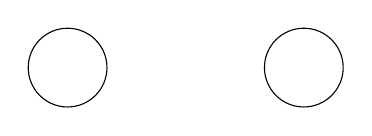
\begin{tikzpicture}
	\draw (0,0) circle (0.5cm);
	\draw (3,0) circle (0.5cm);	
\end{tikzpicture}
\caption{2 bundled conductors}
\end{minipage}
\hspace{0.9cm}
\begin{minipage}[b][][b]{0.3\linewidth}
\begin{tikzpicture}
	\draw (0,0) circle (0.5cm);
	\draw (3,0) circle (0.5cm);
	\draw (1.5,2.598) circle (0.5cm);
\end{tikzpicture}
\caption{3 bundled conductors}
\end{minipage}
\hspace{0.9cm}
\begin{minipage}[b][][b]{0.3\linewidth}
\begin{tikzpicture}
	\draw (0,0) circle (0.5cm);
	\draw (3,0) circle (0.5cm);
	\draw (3,3) circle (0.5cm);
	\draw (0,3) circle (0.5cm);
\end{tikzpicture}
\caption{4 bundled conductors}
\end{minipage}
	
\end{figure}

The calculation of the GMR, or the parameter $D^{b}_{s}$ as it is known for bundle conductors, is exactly the same as that of a stranded conductor. That is to say that each conductor in a bundle is treated as one strand in a conductor. With this in mind, we can use the formula outlined in Problem 2:
\begin{align*}
	GMR = D^{b}_{s} = \sqrt[n^2]{(D_s d_{12} d_{13} ... d_{1n}) ... (D_s d_{n1} d_{n2} ... d_{(n-1)n})}
\end{align*}

We note that in this instance, the $r'$ has been replaced with the $D_s$ of the conductor itself. Hence, for a 2 bundled non-stranded conductor, we see that:
\begin{align*}
	D^{b}_{s} 	&= \sqrt[2^2]{(D_s d_{12})(D_s d_{21})}\\
				&= \sqrt{D_s d}
\end{align*}

For a three bundled non-stranded conductor of equal spacing, we get:
\begin{align*}
	D^{b}_{s}	&= \sqrt[3^2]{(D_S d_{12} d_{13})(D_S d_{21} d_{23})(D_S d_{31} d_{32})}\\
				&= \sqrt[9]{(D_S d^2)(D_S d^2)(D_S d^2)}\\
				&= \sqrt[9]{(D_S d^2)^3}\\
				&= \sqrt[3]{D_S \cdot d^2}
\end{align*}

And finally, for a 4 bundled non-stranded conductor of equal spacing, we get:
\begin{align*}
	D^{b}_{s}	&= \sqrt[4^2]{(D_S d_{12} d_{13} d_{14})(D_S d_{21} d_{23} d_{24})(D_S d_{31} d_{32} d_{34})}\\
				&= \sqrt[16]{(D_S \cdot d \cdot d \cdot \sqrt{2} \cdot d)^4}\\
				&= \sqrt[4]{D_S \cdot d^3 \cdot \sqrt{2}}\\
				&= 1.09 \times \sqrt[4]{D_s \cdot d^3}
\end{align*}
\end{homeworkProblem}

\newpage

\begin{homeworkProblem}
\textbf{Part A}\\
Consider the short line model shown in Figure 13.
\begin{figure}[H]
\centering
\begin{circuitikz}
	\draw (0,0) to [R=$Z$,i=$I_R$,o-o] (5,0);
	\draw (0,-2) to [short,o-o] (5,-2);
	\draw (0,0) to [open,v=$V_S$] (0,-2);
	\draw (5,0) to [open,v^=$V_R$] (5,-2);
\end{circuitikz}
\caption{Short line model.}
\end{figure}
We note that the sending current is equal to the received current, $I_S = I_R$. Further, the the voltage, $V_s$ can be found with the following KVL equation:
\begin{align*}
	V_S = V_R + I_R \cdot Z
\end{align*}

Hence, we get the following matrix equation:
\[
\begin{bmatrix}
	V_S\\
	I_S
\end{bmatrix}
=
\begin{bmatrix}
	1 & Z\\
	0 & 1
\end{bmatrix}
\cdot
\begin{bmatrix}
	V_R\\
	I_R
\end{bmatrix}
\]

Thus, we can see that $A = 1$, $B = Z$, $C = 0$, and $D = 1$.\\

\textbf{Part B}\\
Consider the medium line T-model shown in Figure 14.

\begin{figure}[H]
\centering
\begin{circuitikz}
	\draw (0,0) to [R=$\frac{Z}{2}$,i=$I_S$,o-] (2.5,0)
	to [R=$\frac{Z}{2}$,i=$I_R$,-o] (5,0);
	\draw (2.5,0) to [C] (2.5,-2);
	\draw (0,-2) to [short,o-o] (5,-2);
	\draw (0,0) to [open,v=$V_S$] (0,-2);
	\draw (5,0) to [open,v^=$V_R$] (5,-2);
\end{circuitikz}
\caption{T-model used to model medium length lines.}
\end{figure}


We not that, by KCL, $I_S = I + I_R$, and that $I = Y \cdot V_Y$. Now, substituting the second expression into the first, we get that:
\begin{align*}
	I_S = Y \cdot V_Y + I_R
\end{align*}

Using a KVL in the right most part of the circuit, we see that:
\begin{align*}
	V_Y = V_R + I_R \cdot \frac{Z}{2}
\end{align*}

Hence, substituting the expression for $I_S$ into the expression for $V_Y$, we get that:
\begin{align*}
	I_S &= Y \cdot (V_R + I_R \cdot \frac{Z}{2}) + I_R\\
		&= V_R \cdot Y + (1 + \frac{YZ}{2}) \cdot I_R
\end{align*}

Now, taking a KVL from the left most part of the circuit to the rightmost part of the circuit, skipping the shunt branch, we see that:
\begin{align*}
	V_S &= I_S \cdot \frac{Z}{2} + I_R \cdot \frac{Z}{2} + V_R\\
		&= \bigg(V_R Y + \big[1 + \frac{YZ}{2}\big] I_R \bigg) \cdot \frac{Z}{2} + I_R \frac{Z}{2} + V_R\\
\end{align*}

Rearranging the expression for $V_S$, we see that:
\begin{align*}
	V_S = (1 + \frac{YZ}{2}) \cdot V_R + (Z + \frac{YZ^4}{4}) \cdot I_R
\end{align*}

Hence, the matrix equation for the model is given by:
\[
\begin{bmatrix}
	V_S\\
	I_S
\end{bmatrix}
=
\begin{bmatrix}
	1 + \frac{YZ}{2} & Z + \frac{YZ^2}{4}\\
	Y & 1 + \frac{YZ}{2}
	
\end{bmatrix}
\]

Hence, we see that $A = 1 + \frac{YZ}{2}$, $B = Z + \frac{YZ^2}{4}$, $C = Y$, and $D = 1 + \frac{YZ}{2}$. We note that:
\begin{align*}
	A \cdot D 	&= \big(1 + \frac{YZ}{2}\big) \cdot \big(1 + \frac{YZ}{2}\big)\\
				&= 1 + YZ + \bigg(\frac{YZ}{2}\bigg)^2
\end{align*}

Also, we note that:
\begin{align*}
	BC = YZ + \bigg(\frac{YZ}{2}\bigg)^2
\end{align*}

Hence, we see that $AD \ BC = 1$.\\

\textbf{Part C}\\
Consider the medium line $\pi$-model, shown in Figure 15.

\begin{figure}[H]
\centering
\begin{circuitikz}
	\draw (0,0) to [short,i=$I_S$,o-] (1,0)
	to [R=$Z$] (4,0)
	to [short,i=$I_R$,-o] (5,0);
	\draw (1,0) to [C=$\frac{Y}{2}$] (1,-2);
	\draw (4,0) to [C=$\frac{Y}{2}$] (4,-2);
	\draw (0,-2) to [short,o-o] (5,-2);
	\draw (0,0) to [open,v=$V_S$] (0,-2);
	\draw (5,0) to [open,v^=$V_R$] (5,-2);
\end{circuitikz}
\caption{T-model used to model medium length lines.}
\end{figure}

We note that the current across the impedance $Z$, denoted as $I$, is given by $I = I_R + V_R \cdot \frac{Y}{2}$. Now, taking a KVL around the full circuit, we see that:
\begin{align*}
	V_S &= V_R + I \cdot Z\\
		&= V_R + (I_R + V_R) \cdot Z\\
		&= \bigg( 1 + \frac{YZ}{2} \bigg) \cdot V_R + Z \cdot I_R
\end{align*}

We also note, that by KCL on the left most node in the circuit, we get:
\begin{align*}
	I_S &= \frac{Y}{2} \cdot V_S + I\\
		&= \frac{Y}{2} \cdot \bigg(V_R + I_R \cdot Z + V_R \cdot \frac{YZ}{2}\bigg) + I_R + V_R \cdot \frac{Y}{2}
\end{align*}

Rearranging, we get that:
\begin{align*}
	I_S = \bigg(Y + \frac{Y^2 Z}{4}\bigg) \cdot V_R + \bigg(1 + \frac{YZ}{2}\bigg) \cdot I_R
\end{align*}

Hence, the matrix equation of the model is given by:
\[
\begin{bmatrix}
	V_S\\
	I_S
\end{bmatrix}
=
\begin{bmatrix}
	1 + \sfrac{YZ}{2} & Z\\
	Y + \sfrac{Y^2 Z}{4} & 1 + \sfrac{YZ}{2}
\end{bmatrix}
\cdot
\begin{bmatrix}
	V_R\\
	I_R
\end{bmatrix}
\]

Hence, we see that:
\begin{align*}
	AD 	&= (1 + \frac{YZ}{2})(1 + \frac{YZ}{2})\\
		&= 1 + YZ + \bigg(\frac{YZ}{2}\bigg)^2
\end{align*}

Further, we see that:
\begin{align*}
	BC 	&= Z \cdot \bigg( Y + \frac{Y^2 Z}{4} \bigg)\\
		&= YZ + \bigg(\frac{YZ}{2}\bigg)^2
\end{align*}

Hence, we find that $AD - BC = 1$.\\

\textbf{Part D}\\
Consider the long line model shown in Figure 16.

\begin{figure}[H]
\centering
	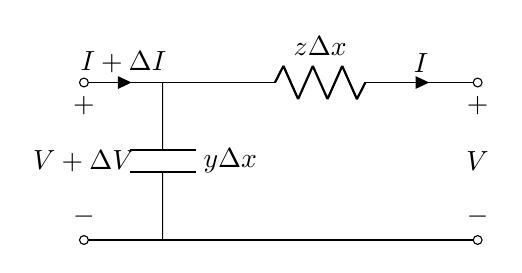
\begin{tikzpicture}
		\draw (0,0) to [short,i=$I + \Delta I$,o-] (1,0)
		to [R=$z \Delta x$,i=$I$,-o] (5,0);
		\draw (1,0) to [C=$y \Delta x$] (1,-2);
		\draw (0,-2) to [short,o-o] (5,-2);
		\draw (0,0) to [open,v=$V + \Delta V$] (0,-2);
		\draw (5,0) to [open,v^=$V$] (5,-2);
	\end{tikzpicture}
\end{figure}

This figure depicts a small strip $\Delta x$ that is a distance of $x$ from the receiving end of the strip. The voltage and current at the receiving end of the strip are $V$ and $I$. At the beginning of the strip the voltage and current are $V + \Delta V$ and $I + \Delta I$. The voltage drop across the strip is then $\Delta V$. The length of the strip is $\Delta x$, the series impedance and the shunt admittance are given by $z \cdot \Delta x$ and $y \cdot \Delta x$, where $z$ and $y$ are the impedance and admittance per unit length. We also note that, given the length of the line, $l$, that the full impedance and full admittance are given by:
\begin{align*}
	Z 	&= z \times l\\
	Y	&= y \times l
\end{align*}

Now, from the circuit, we see that:
\begin{align*}
	\Delta V &= I \cdot (z \cdot \Delta x)\\
	\implies \frac{\Delta V}{\Delta x} &= I \cdot z
\end{align*}

As we shrink the strip to an infinitesimally small strip, we take the limit $\Delta x \rightarrow 0$. Hence, we see that:
\begin{align*}
	\lim_{\Delta x \rightarrow 0} \frac{\Delta V}{\Delta x} &= I \cdot z\\
	\implies \frac{dV}{dx} &= I \cdot z
\end{align*}

Considering the current through the strip, we see that:
\begin{align*}
	\Delta I = (V + \Delta V) \cdot (y \Delta x) = V \cdot (y \Delta x) + \Delta V \cdot (y \Delta x)
\end{align*}

Since the second term in the equation is the multiplication of two small values, the resultant is very small and we can neglect its contribution to the equation. Hence, we see that:
\begin{align*}
	\frac{\Delta I}{\Delta x} = Vy
\end{align*}

Considering an infintesimailly small strip we take the limit as $\Delta x \rightarrow 0$ and get:
\begin{align*}
	\lim_{\Delta x \rightarrow 0} \frac{\Delta I}{\Delta x} &= Vy\\
	\implies \frac{dI}{dx} &= Vy
\end{align*}

Now, taking the derivative of the first differential equation, we get that:
\begin{align*}
	\frac{d}{dx} \bigg(\frac{dV}{dx}\bigg) &= z \frac{dI}{dx}\\
	\frac{d^2 V}{dx^2} &= zyV
\end{align*}

Rearranging, we get the differential equation:
\begin{align*}
	\frac{d^2 V}{d x^2} - zyV = 0
\end{align*}

We note that the characteristic equation of the ODE is given by:
\begin{align*}
	\lambda^2 - zy = 0
\end{align*}

Hence, we see the roots of the characteristic polynomial are $\lambda_{1,2} = \pm \sqrt{zy}$, and the general solution to the homogeneous ODE is given by:
\begin{align*}
	V = A_1 \cdot e^{x \sqrt{zy}} + A_2 \cdot e^{-x \sqrt{zy}}
\end{align*}

Taking the derivative of this equation, with respect to $x$, we get:
\begin{align*}
	\frac{dV}{dx} = A_1 \cdot \sqrt{yz} \cdot e^{x \sqrt{zy}} - A_2 \cdot \sqrt{yz} \cdot e^{-x \sqrt{zy}}
\end{align*}

We can derive an expression for the current, $I$, using a the first differential expression we derived, $\frac{dV}{dx} = I \cdot z$. Hence, we see that:
\begin{align*}
	I 	&= \frac{1}{z} \cdot \bigg(\frac{dV}{dx}\bigg)\\
		&= \frac{A_1}{\sqrt{\sfrac{z}{y}}} \cdot e^{x \sqrt{yz}} - \frac{A_2}{\sqrt{\sfrac{z}{y}}} \cdot e^{-x \sqrt{yz}} 
\end{align*}

By defining two variables, we can simplify the above expressions. We define the characteristic impedance, $Z_C$, and the propagation constant, $\gamma$. The definitions are as follow:
\begin{align*}
	Z_C &= \sqrt{\frac{z}{y}} \si{\ohm}
	\gamma &= \sqrt{zy}
\end{align*}

Hence, we simplify the expression for voltage, $V$:
\begin{align*}
	V = A_1 \cdot e^{\gamma x} + A_2 \cdot e^{- \gamma x} 
\end{align*}

And we simplify the expression for current, $I$:
\begin{align*}
	I = \frac{A_1}{Z_C} \cdot e^{\gamma x} - \frac{A_2}{Z_C} \cdot e^{- \gamma x}
\end{align*}

Now we consider the boundary conditions in turn, $x = 0$, and $x = l$. First, lets consider $x = 0$. We note that in this case, $V = V_R$ and $I = I_R$, hence we get:
\begin{align*}
	V_R &= A_1 + A_2\\
	I_R &= \frac{A_1}{Z_C} - \frac{A_2}{Z_C}
\end{align*}

Solving the simultaneous equations for $A_1$ and $A_2$, we get that:
\begin{align*}
	A_1 &= \frac{V_R + Z_C I_R}{2}\\
	A_2 &= \frac{V_R - Z_CI_R}{2}
\end{align*}

Considering the other boundary condition, $x = l$, we see note that $V = V_S$ and $I = I_S$, and hence, we write the expressions including the constant terms $A_1$ and $A_2$ as:
\begin{align*}
	V_S &= \frac{V_R + Z_C I_R}{2} \cdot e^{\gamma l} + \frac{V_R - Z_C I_R}{2} \cdot e^{-\gamma l}\\
	I_S = &= \frac{\sfrac{V_R}{Z_C} + I_R}{2} \cdot e^{\gamma l} - \frac{\sfrac{V_R}{Z_C} - I_R}{2} \cdot e^{-\gamma l}
\end{align*}

Noting that we can express the exponentials as hyperbolic trigonometric functions we obtain the final expressions:
\begin{align*}
	V_S &= V_R \cdot \cosh (\gamma l) + Z_C I_R \cdot \sinh (\gamma l)\\
	I_S &= V_R \cdot \frac{1}{Z_C} \cdot \sinh (\gamma l) + I_R \cdot \cosh (\gamma l)
\end{align*}

Finally, we can write this in the matrix form as follows:
\[
\begin{bmatrix}
	V_S\\
	I_S
\end{bmatrix}
=
\begin{bmatrix}
	\cosh (\gamma l) & Z_C \cdot \sinh (\gamma l)\\
	\frac{1}{Z_C} \cdot \sinh (\gamma l) & \cosh (\gamma l)
\end{bmatrix}
\cdot
\begin{bmatrix}
	V_R\\
	I_R
\end{bmatrix}
\]

We see that $A = D = \cosh (\gamma l)$, $B = Z_C \cdot \sinh(\gamma l)$, and $C = \frac{1}{Z_C} \cdot \sinh (\gamma l)$. Finally, we note that:
\begin{align*}
	AD = \cosh^2 (\gamma l)
\end{align*}

And that:
\begin{align*}
	BC = \sinh^2 (\gamma l)
\end{align*}

Hence, we see that $AD - BC = \cosh^2 (\gamma l) - \sinh^2 (\gamma l) = 1$
\end{homeworkProblem}
\end{document}
